\documentclass[11pt,]{article}
\usepackage{lmodern}
\usepackage{amssymb,amsmath}
\usepackage{ifxetex,ifluatex}
\usepackage{fixltx2e} % provides \textsubscript
\ifnum 0\ifxetex 1\fi\ifluatex 1\fi=0 % if pdftex
  \usepackage[T1]{fontenc}
  \usepackage[utf8]{inputenc}
\else % if luatex or xelatex
  \ifxetex
    \usepackage{mathspec}
  \else
    \usepackage{fontspec}
  \fi
  \defaultfontfeatures{Ligatures=TeX,Scale=MatchLowercase}
\fi
% use upquote if available, for straight quotes in verbatim environments
\IfFileExists{upquote.sty}{\usepackage{upquote}}{}
% use microtype if available
\IfFileExists{microtype.sty}{%
\usepackage{microtype}
\UseMicrotypeSet[protrusion]{basicmath} % disable protrusion for tt fonts
}{}
\usepackage[margin=1in]{geometry}
\usepackage{hyperref}
\PassOptionsToPackage{usenames,dvipsnames}{color} % color is loaded by hyperref
\hypersetup{unicode=true,
            colorlinks=true,
            linkcolor=black,
            citecolor=Blue,
            urlcolor=black,
            breaklinks=true}
\urlstyle{same}  % don't use monospace font for urls
\usepackage{color}
\usepackage{fancyvrb}
\newcommand{\VerbBar}{|}
\newcommand{\VERB}{\Verb[commandchars=\\\{\}]}
\DefineVerbatimEnvironment{Highlighting}{Verbatim}{commandchars=\\\{\}}
% Add ',fontsize=\small' for more characters per line
\usepackage{framed}
\definecolor{shadecolor}{RGB}{248,248,248}
\newenvironment{Shaded}{\begin{snugshade}}{\end{snugshade}}
\newcommand{\KeywordTok}[1]{\textcolor[rgb]{0.13,0.29,0.53}{\textbf{{#1}}}}
\newcommand{\DataTypeTok}[1]{\textcolor[rgb]{0.13,0.29,0.53}{{#1}}}
\newcommand{\DecValTok}[1]{\textcolor[rgb]{0.00,0.00,0.81}{{#1}}}
\newcommand{\BaseNTok}[1]{\textcolor[rgb]{0.00,0.00,0.81}{{#1}}}
\newcommand{\FloatTok}[1]{\textcolor[rgb]{0.00,0.00,0.81}{{#1}}}
\newcommand{\ConstantTok}[1]{\textcolor[rgb]{0.00,0.00,0.00}{{#1}}}
\newcommand{\CharTok}[1]{\textcolor[rgb]{0.31,0.60,0.02}{{#1}}}
\newcommand{\SpecialCharTok}[1]{\textcolor[rgb]{0.00,0.00,0.00}{{#1}}}
\newcommand{\StringTok}[1]{\textcolor[rgb]{0.31,0.60,0.02}{{#1}}}
\newcommand{\VerbatimStringTok}[1]{\textcolor[rgb]{0.31,0.60,0.02}{{#1}}}
\newcommand{\SpecialStringTok}[1]{\textcolor[rgb]{0.31,0.60,0.02}{{#1}}}
\newcommand{\ImportTok}[1]{{#1}}
\newcommand{\CommentTok}[1]{\textcolor[rgb]{0.56,0.35,0.01}{\textit{{#1}}}}
\newcommand{\DocumentationTok}[1]{\textcolor[rgb]{0.56,0.35,0.01}{\textbf{\textit{{#1}}}}}
\newcommand{\AnnotationTok}[1]{\textcolor[rgb]{0.56,0.35,0.01}{\textbf{\textit{{#1}}}}}
\newcommand{\CommentVarTok}[1]{\textcolor[rgb]{0.56,0.35,0.01}{\textbf{\textit{{#1}}}}}
\newcommand{\OtherTok}[1]{\textcolor[rgb]{0.56,0.35,0.01}{{#1}}}
\newcommand{\FunctionTok}[1]{\textcolor[rgb]{0.00,0.00,0.00}{{#1}}}
\newcommand{\VariableTok}[1]{\textcolor[rgb]{0.00,0.00,0.00}{{#1}}}
\newcommand{\ControlFlowTok}[1]{\textcolor[rgb]{0.13,0.29,0.53}{\textbf{{#1}}}}
\newcommand{\OperatorTok}[1]{\textcolor[rgb]{0.81,0.36,0.00}{\textbf{{#1}}}}
\newcommand{\BuiltInTok}[1]{{#1}}
\newcommand{\ExtensionTok}[1]{{#1}}
\newcommand{\PreprocessorTok}[1]{\textcolor[rgb]{0.56,0.35,0.01}{\textit{{#1}}}}
\newcommand{\AttributeTok}[1]{\textcolor[rgb]{0.77,0.63,0.00}{{#1}}}
\newcommand{\RegionMarkerTok}[1]{{#1}}
\newcommand{\InformationTok}[1]{\textcolor[rgb]{0.56,0.35,0.01}{\textbf{\textit{{#1}}}}}
\newcommand{\WarningTok}[1]{\textcolor[rgb]{0.56,0.35,0.01}{\textbf{\textit{{#1}}}}}
\newcommand{\AlertTok}[1]{\textcolor[rgb]{0.94,0.16,0.16}{{#1}}}
\newcommand{\ErrorTok}[1]{\textcolor[rgb]{0.64,0.00,0.00}{\textbf{{#1}}}}
\newcommand{\NormalTok}[1]{{#1}}
\usepackage{graphicx,grffile}
\makeatletter
\def\maxwidth{\ifdim\Gin@nat@width>\linewidth\linewidth\else\Gin@nat@width\fi}
\def\maxheight{\ifdim\Gin@nat@height>\textheight\textheight\else\Gin@nat@height\fi}
\makeatother
% Scale images if necessary, so that they will not overflow the page
% margins by default, and it is still possible to overwrite the defaults
% using explicit options in \includegraphics[width, height, ...]{}
\setkeys{Gin}{width=\maxwidth,height=\maxheight,keepaspectratio}
\IfFileExists{parskip.sty}{%
\usepackage{parskip}
}{% else
\setlength{\parindent}{0pt}
\setlength{\parskip}{6pt plus 2pt minus 1pt}
}
\setlength{\emergencystretch}{3em}  % prevent overfull lines
\providecommand{\tightlist}{%
  \setlength{\itemsep}{0pt}\setlength{\parskip}{0pt}}
\setcounter{secnumdepth}{5}
% Redefines (sub)paragraphs to behave more like sections
\ifx\paragraph\undefined\else
\let\oldparagraph\paragraph
\renewcommand{\paragraph}[1]{\oldparagraph{#1}\mbox{}}
\fi
\ifx\subparagraph\undefined\else
\let\oldsubparagraph\subparagraph
\renewcommand{\subparagraph}[1]{\oldsubparagraph{#1}\mbox{}}
\fi

%%% Use protect on footnotes to avoid problems with footnotes in titles
\let\rmarkdownfootnote\footnote%
\def\footnote{\protect\rmarkdownfootnote}

%%% Change title format to be more compact
\usepackage{titling}

% Create subtitle command for use in maketitle
\newcommand{\subtitle}[1]{
  \posttitle{
    \begin{center}\large#1\end{center}
    }
}

\setlength{\droptitle}{-2em}
  \title{}
  \pretitle{\vspace{\droptitle}}
  \posttitle{}
  \author{}
  \preauthor{}\postauthor{}
  \date{}
  \predate{}\postdate{}

\usepackage{lineno}
\linenumbers
\usepackage{setspace}
\usepackage{todonotes}
\onehalfspacing
\usepackage{rotating}
\usepackage{color, soul}
\usepackage[font={normalsize},labelfont={bf},labelsep=quad]{caption}
\usepackage{tikz}

\begin{document}

\newcommand{\tikzcircle}[2][red,fill=red]{\tikz[baseline=-0.5ex]\draw[#1,radius=#2] (0,0) circle ;}
\renewcommand\linenumberfont{\normalfont\tiny\sffamily\color{gray}}
\renewcommand\thefigure{S1-\arabic{figure}}  
\renewcommand\thetable{S1-\arabic{table}}  
\renewcommand\thesection{Section SI.\arabic{section}}

\begin{center}
\textbf{\Large{Supporting Information}} \\
A.T. Tredennick, P.B. Adler, \& F.R. Adler, ``The relationship between species richness and...'' \\
\emph{Ecology Letters}
\end{center}

\section{R Code for Consumer-Resource Model}

Below is the R code for our model function, which is represented
mathematically in the main text in Equations 1-4. The same code, along
with all the code to reproduce our results, has been archived on
Figshare (link) and is available on GitHub
(\url{http://github.com/atredennick/Coexistence-Stability/releases}).

\begin{Shaded}
\begin{Highlighting}[]
\NormalTok{simulate_model <-}\StringTok{ }\NormalTok{function(seasons, days_to_track, Rmu, }
                           \NormalTok{Rsd_annual, sigE, rho, }
                           \NormalTok{alpha1, alpha2, alpha3, alpha4,}
                           \NormalTok{eta1, eta2, eta3, eta4,}
                           \NormalTok{r1, r2, r3, r4,}
                           \NormalTok{a1, a2, a3, a4,}
                           \NormalTok{b1, b2, b3, b4,}
                           \NormalTok{eps1, eps2, eps3, eps4,}
                           \NormalTok{D1, D2, D3, D4,}
                           \NormalTok{N1, N2, N3, N4, R) \{}
  
  \KeywordTok{require}\NormalTok{(}\StringTok{'deSolve'}\NormalTok{) }\CommentTok{# for solving continuous differential equations}
  \KeywordTok{require}\NormalTok{(}\StringTok{'mvtnorm'}\NormalTok{) }\CommentTok{# for multivariate normal distribution functions}
  
  \NormalTok{##  Assign parameter values to appropriate lists}
  \NormalTok{DNR <-}\StringTok{ }\KeywordTok{c}\NormalTok{(}\DataTypeTok{D=}\KeywordTok{c}\NormalTok{(D1,D2,D3,D4),   }\CommentTok{# initial dormant state abundance}
           \DataTypeTok{N=}\KeywordTok{c}\NormalTok{(N1,N2,N3,N4),   }\CommentTok{# initial live state abundance}
           \DataTypeTok{R=}\NormalTok{R)                }\CommentTok{# initial resource level}
  
  \NormalTok{parms <-}\StringTok{ }\KeywordTok{list} \NormalTok{(}
    \DataTypeTok{r   =} \KeywordTok{c}\NormalTok{(r1,r2,r3,r4),          }\CommentTok{# max growth rate for each species}
    \DataTypeTok{a   =} \KeywordTok{c}\NormalTok{(a1,a2,a3,a4),          }\CommentTok{# rate parameter for Hill function }
    \DataTypeTok{b   =} \KeywordTok{c}\NormalTok{(b1,b2,b3,b4),          }\CommentTok{# shape parameter for Hill function}
    \DataTypeTok{eps =} \KeywordTok{c}\NormalTok{(eps1,eps2,eps3,eps4)   }\CommentTok{# resource-to-biomass efficiency}
  \NormalTok{)}
  
  
  \NormalTok{####}
  \NormalTok{####  Sub-Model functions ----------------------------------------------------}
  \NormalTok{####}
  \NormalTok{## Continuous model}
  \NormalTok{updateNR <-}\StringTok{ }\NormalTok{function(t, NR, parms)\{}
    \KeywordTok{with}\NormalTok{(}\KeywordTok{as.list}\NormalTok{(}\KeywordTok{c}\NormalTok{(NR, parms)), \{}
      \NormalTok{dN1dt =}\StringTok{ }\NormalTok{N1*eps[}\DecValTok{1}\NormalTok{]*(}\KeywordTok{uptake_R}\NormalTok{(r[}\DecValTok{1}\NormalTok{], R, a[}\DecValTok{1}\NormalTok{], b[}\DecValTok{1}\NormalTok{]))}
      \NormalTok{dN2dt =}\StringTok{ }\NormalTok{N2*eps[}\DecValTok{2}\NormalTok{]*(}\KeywordTok{uptake_R}\NormalTok{(r[}\DecValTok{2}\NormalTok{], R, a[}\DecValTok{2}\NormalTok{], b[}\DecValTok{2}\NormalTok{]))}
      \NormalTok{dN3dt =}\StringTok{ }\NormalTok{N3*eps[}\DecValTok{3}\NormalTok{]*(}\KeywordTok{uptake_R}\NormalTok{(r[}\DecValTok{3}\NormalTok{], R, a[}\DecValTok{3}\NormalTok{], b[}\DecValTok{3}\NormalTok{]))}
      \NormalTok{dN4dt =}\StringTok{ }\NormalTok{N4*eps[}\DecValTok{4}\NormalTok{]*(}\KeywordTok{uptake_R}\NormalTok{(r[}\DecValTok{4}\NormalTok{], R, a[}\DecValTok{4}\NormalTok{], b[}\DecValTok{4}\NormalTok{]))}
      \NormalTok{dRdt  =}\StringTok{ }\NormalTok{-}\DecValTok{1} \NormalTok{*}\StringTok{ }\NormalTok{(dN1dt/eps[}\DecValTok{1}\NormalTok{] +}\StringTok{ }\NormalTok{dN2dt/eps[}\DecValTok{2}\NormalTok{] +}\StringTok{ }\NormalTok{dN3dt/eps[}\DecValTok{3}\NormalTok{] +}\StringTok{ }\NormalTok{dN4dt/eps[}\DecValTok{4}\NormalTok{])}
      \KeywordTok{list}\NormalTok{(}\KeywordTok{c}\NormalTok{(dN1dt, dN2dt, dN3dt, dN4dt, dRdt)) }\CommentTok{# output as list}
    \NormalTok{\})}
  \NormalTok{\} }\CommentTok{# end continuous function}
  
  \NormalTok{## Discrete model}
  \NormalTok{update_DNR <-}\StringTok{ }\NormalTok{function(t, DNR, gammas,}
                         \NormalTok{alpha1, alpha2, alpha3, alpha4,}
                         \NormalTok{eta1, eta2, eta3, eta4) \{}
    \KeywordTok{with} \NormalTok{(}\KeywordTok{as.list}\NormalTok{(DNR),\{}
      \NormalTok{g1    <-}\StringTok{ }\NormalTok{gammas[}\DecValTok{1}\NormalTok{]}
      \NormalTok{g2    <-}\StringTok{ }\NormalTok{gammas[}\DecValTok{2}\NormalTok{]}
      \NormalTok{g3    <-}\StringTok{ }\NormalTok{gammas[}\DecValTok{3}\NormalTok{]}
      \NormalTok{g4    <-}\StringTok{ }\NormalTok{gammas[}\DecValTok{4}\NormalTok{]}
      \NormalTok{D1new <-}\StringTok{ }\NormalTok{(}\DecValTok{1}\NormalTok{-g1)*(alpha1*N1 +}\StringTok{ }\NormalTok{D1)*(}\DecValTok{1}\NormalTok{-eta1)}
      \NormalTok{D2new <-}\StringTok{ }\NormalTok{(}\DecValTok{1}\NormalTok{-g2)*(alpha2*N2 +}\StringTok{ }\NormalTok{D2)*(}\DecValTok{1}\NormalTok{-eta2)}
      \NormalTok{D3new <-}\StringTok{ }\NormalTok{(}\DecValTok{1}\NormalTok{-g3)*(alpha3*N3 +}\StringTok{ }\NormalTok{D3)*(}\DecValTok{1}\NormalTok{-eta3)}
      \NormalTok{D4new <-}\StringTok{ }\NormalTok{(}\DecValTok{1}\NormalTok{-g4)*(alpha4*N4 +}\StringTok{ }\NormalTok{D4)*(}\DecValTok{1}\NormalTok{-eta4)}
      \NormalTok{N1new <-}\StringTok{ }\NormalTok{g1*(alpha1*N1 +}\StringTok{ }\NormalTok{D1)*(}\DecValTok{1}\NormalTok{-eta1)}
      \NormalTok{N2new <-}\StringTok{ }\NormalTok{g2*(alpha2*N2 +}\StringTok{ }\NormalTok{D2)*(}\DecValTok{1}\NormalTok{-eta2)}
      \NormalTok{N3new <-}\StringTok{ }\NormalTok{g3*(alpha3*N3 +}\StringTok{ }\NormalTok{D3)*(}\DecValTok{1}\NormalTok{-eta3)}
      \NormalTok{N4new <-}\StringTok{ }\NormalTok{g4*(alpha4*N4 +}\StringTok{ }\NormalTok{D4)*(}\DecValTok{1}\NormalTok{-eta4)}
      \NormalTok{Rnew  <-}\StringTok{ }\NormalTok{Rvector[t]}
      \KeywordTok{return}\NormalTok{(}\KeywordTok{c}\NormalTok{(D1new, D2new, D3new, D4new, N1new, N2new, N3new, N4new, Rnew))}
    \NormalTok{\})}
  \NormalTok{\}}
  
  \NormalTok{##  Resource uptake function (Hill function)}
  \NormalTok{uptake_R <-}\StringTok{ }\NormalTok{function(r, R, a, b) \{}
    \KeywordTok{return}\NormalTok{((r*R^a) /}\StringTok{ }\NormalTok{(b^a +}\StringTok{ }\NormalTok{R^a))}
  \NormalTok{\}}
  
  \NormalTok{##  Generate germination fractions}
  \NormalTok{getG <-}\StringTok{ }\NormalTok{function(sigE, rho, nTime, num_spp) \{}
    \NormalTok{varcov       <-}\StringTok{ }\KeywordTok{matrix}\NormalTok{(}\KeywordTok{rep}\NormalTok{(rho*sigE,num_spp*}\DecValTok{2}\NormalTok{), num_spp, num_spp)}
    \KeywordTok{diag}\NormalTok{(varcov) <-}\StringTok{ }\NormalTok{sigE}
    \NormalTok{if(sigE >}\StringTok{ }\DecValTok{0}\NormalTok{) \{ varcov <-}\StringTok{ }\NormalTok{Matrix::}\KeywordTok{nearPD}\NormalTok{(varcov)$mat \} }\CommentTok{# crank through nearPD to fix rounding errors }
    \NormalTok{varcov <-}\StringTok{ }\KeywordTok{as.matrix}\NormalTok{(varcov)}
    \NormalTok{e      <-}\StringTok{ }\KeywordTok{rmvnorm}\NormalTok{(}\DataTypeTok{n =} \NormalTok{nTime, }\DataTypeTok{mean =} \KeywordTok{rep}\NormalTok{(}\DecValTok{0}\NormalTok{,num_spp), }\DataTypeTok{sigma =} \NormalTok{varcov)}
    \NormalTok{g      <-}\StringTok{ }\KeywordTok{exp}\NormalTok{(e) /}\StringTok{ }\NormalTok{(}\DecValTok{1}\NormalTok{+}\KeywordTok{exp}\NormalTok{(e))}
    \KeywordTok{return}\NormalTok{(g)}
  \NormalTok{\}}
  
  
  \NormalTok{####}
  \NormalTok{#### Simulate model -----------------------------------------------------}
  \NormalTok{####}
  \NormalTok{days           <-}\StringTok{ }\KeywordTok{c}\NormalTok{(}\DecValTok{1}\NormalTok{:days_to_track)}
  \NormalTok{num_spp        <-}\StringTok{ }\KeywordTok{length}\NormalTok{(parms$r)}
  \NormalTok{nmsDNR         <-}\StringTok{ }\KeywordTok{names}\NormalTok{(DNR)}
  \NormalTok{dormants       <-}\StringTok{ }\KeywordTok{grep}\NormalTok{(}\StringTok{"D"}\NormalTok{, }\KeywordTok{names}\NormalTok{(DNR))}
  \NormalTok{NR             <-}\StringTok{ }\NormalTok{DNR[-dormants] }
  \NormalTok{nmsNR          <-}\StringTok{ }\KeywordTok{names}\NormalTok{(NR)}
  \NormalTok{gVec           <-}\StringTok{ }\KeywordTok{getG}\NormalTok{(}\DataTypeTok{sigE =} \NormalTok{sigE, }\DataTypeTok{rho =} \NormalTok{rho, }\DataTypeTok{nTime =} \NormalTok{seasons, }\DataTypeTok{num_spp =} \NormalTok{num_spp)}
  \NormalTok{Rvector        <-}\StringTok{ }\KeywordTok{rlnorm}\NormalTok{(seasons, Rmu, Rsd_annual)}
  \NormalTok{saved_outs     <-}\StringTok{ }\KeywordTok{matrix}\NormalTok{(}\DataTypeTok{ncol=}\KeywordTok{length}\NormalTok{(DNR), }\DataTypeTok{nrow=}\NormalTok{seasons}\DecValTok{+1}\NormalTok{)}
  \NormalTok{saved_outs[}\DecValTok{1}\NormalTok{,] <-}\StringTok{ }\NormalTok{DNR }

  \NormalTok{##  Loop over seasons}
  \NormalTok{for(season_now in }\DecValTok{1}\NormalTok{:seasons) \{}
    \CommentTok{# Simulate continuous growing  season}
    \NormalTok{output   <-}\StringTok{ }\KeywordTok{ode}\NormalTok{(}\DataTypeTok{y =} \NormalTok{NR, }\DataTypeTok{times=}\NormalTok{days, }\DataTypeTok{func =} \NormalTok{updateNR, }\DataTypeTok{parms =} \NormalTok{parms)}
    \NormalTok{NR       <-}\StringTok{ }\NormalTok{output[}\KeywordTok{nrow}\NormalTok{(output),nmsNR]}
    \NormalTok{dormants <-}\StringTok{ }\KeywordTok{grep}\NormalTok{(}\StringTok{"D"}\NormalTok{, }\KeywordTok{names}\NormalTok{(DNR)) }
    \NormalTok{DNR      <-}\StringTok{ }\KeywordTok{c}\NormalTok{(DNR[dormants], NR)}
    
    \CommentTok{# Save end of season biomasses, before discrete transitions}
    \NormalTok{saved_outs[season_now}\DecValTok{+1}\NormalTok{,] <-}\StringTok{ }\NormalTok{DNR}
    
    \KeywordTok{names}\NormalTok{(DNR) <-}\StringTok{ }\NormalTok{nmsDNR}
    \NormalTok{DNR        <-}\StringTok{ }\KeywordTok{update_DNR}\NormalTok{(season_now, DNR, gVec[season_now,],}
                             \DataTypeTok{alpha1 =} \NormalTok{alpha1, }\DataTypeTok{alpha2 =} \NormalTok{alpha2, }
                             \DataTypeTok{alpha3 =} \NormalTok{alpha3, }\DataTypeTok{alpha4 =} \NormalTok{alpha4,}
                             \DataTypeTok{eta1 =} \NormalTok{eta1, }\DataTypeTok{eta2 =} \NormalTok{eta2, }\DataTypeTok{eta3 =} \NormalTok{eta3, }\DataTypeTok{eta4 =} \NormalTok{eta4)}
    
    \KeywordTok{names}\NormalTok{(DNR) <-}\StringTok{ }\NormalTok{nmsDNR}
    \NormalTok{NR         <-}\StringTok{ }\NormalTok{DNR[-dormants]  }
    \KeywordTok{names}\NormalTok{(NR)  <-}\StringTok{ }\NormalTok{nmsNR}
  \NormalTok{\} }\CommentTok{# next season}
  
  \KeywordTok{return}\NormalTok{(saved_outs)}
  
\NormalTok{\} }\CommentTok{#end simulation function}
\end{Highlighting}
\end{Shaded}

\section{Exploring Parameter Space}

\section{Eight-Species Storage Effect Model}

In the main text we constrained our focus to four-species communities
because getting more than four species to coexist by relative
nonlinearity is tricky, and usually requires adding another coexistence
mechanism on top off relative nonlinearity (Yuan \& Chesson 2015). The
storage effect does not suffer from this limitation, but we wanted our
results in the main text to be easily comparable between coexistence
mechanisms. Here, we show that our results are qualitatively similar if
we simulate an eight-species community with species coexistence
maintained by the storage effect. We conducted the same numerical
simulations described in the main text for Figure 2. Quoting from the
main text:

\begin{quote}
\emph{First, we allowed the variance of the environment to determine how many species can coexist, akin to a community assembly experiment with a species pool of four species.
To do this, we simulated communities with all species initially present across a gradient of annual resource variability (for relative nonlinearity) or environmental cue variability (for the storage effect).
Second, we chose parameter values that allowed coexistence of all four species and then performed species removals, akin to a biodiversity--ecosystem function experiment.
The two simulation experiments correspond to (i) sampling ecosystem function across a natural gradient of species richness and (ii) sampling ecosystem function across diversity treatments within a site.}
\end{quote}

From one to four species, the relationship is as presented in the main
text: total community \emph{CV} increases approximately linearly with
environmental variability because (1) environmental variability promotes
species coexistence \emph{and} (2) environmental variability causes
populations fluctuations to increase (Figure S1-1). However, after four
species, the relationship saturates --- species additions due to
coexistence by the storage effect completely buffer ecosystem
variability from further increases in environmental variability (Figure
S1-1). Thus, our results provide novel theoretical explanations for
positive and flat diversity--ecosystem variability relationships.

\begin{figure}[!ht]
  \centering
      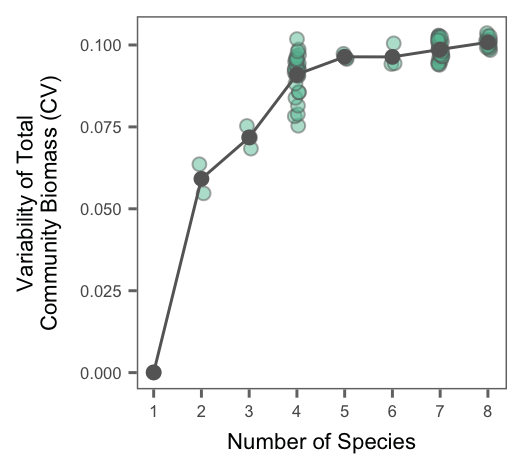
\includegraphics[width=4in]{./components/regional_diversity_stability_storage_effect_8species.png}
  \caption{A storage effect result.}
\end{figure}

\newpage{}

\section{Additional Figures}

\begin{figure}[!ht]
  \centering
      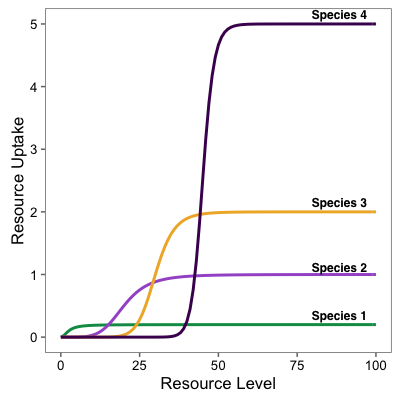
\includegraphics[width=3in]{./components/fourspp_Ruptake_relnonlin.png}
  \caption{Resource uptake curves for each species (represented by different colors) as used in relative nonlinearity simulations. The equation for resource uptake is: $f_{i}(R) = r_{i}R^{a_{i}} / (b_{i}^{a_{i}}+R^{a_{i}})$. Parameter values are as follows. Species 1: \emph{r} = 0.2, \emph{a} = 2, \emph{b} = 2.5; Species 2: \emph{r} = 1, \emph{a} = 5, \emph{b} = 20; Species 3: \emph{r} = 2, \emph{a} = 10, \emph{b} = 30; Species 4: \emph{r} = 5, \emph{a} = 25, \emph{b} = 45.}
\end{figure}

\newpage{}

\begin{figure}[!ht]
  \centering
      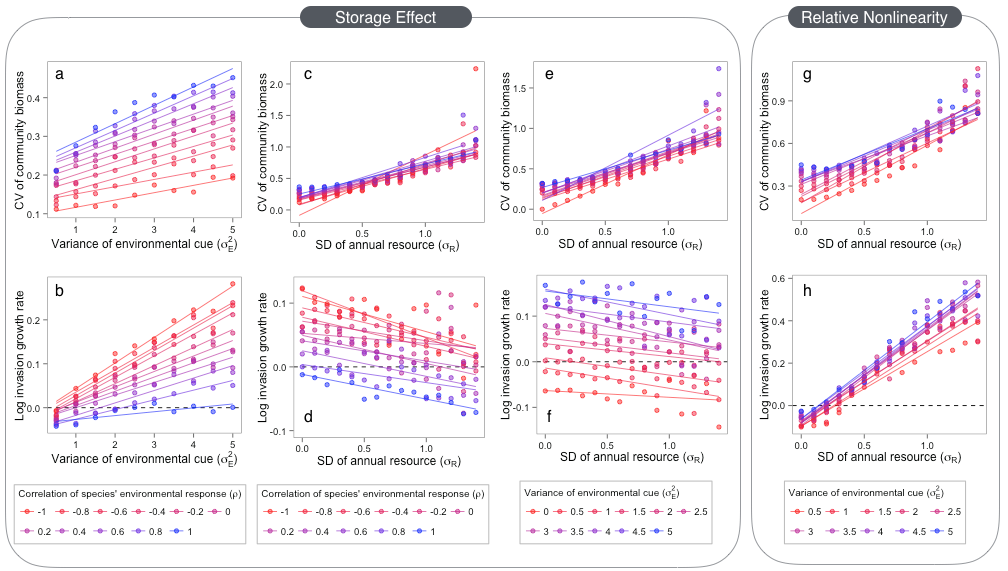
\includegraphics[width=4in]{./components/SI_invasion_factorials.png}
  \caption{Variability of community biomass and invasion growth rates of the inferior competitor in a two-species community under different parameter combinations. Points are mean values from 5,000 growing seasons and lines are linear fits to show trends. In \textbf{Storage Effect} plots (a,b), resource supply is held constant between growing seasons. Resource supply varies each year in \textbf{Relative Nonlinearity} simulations (c,d), while the environmental cue variance is set to 0.}
\end{figure}

\newpage{}

\begin{figure}[!ht]
  \centering
      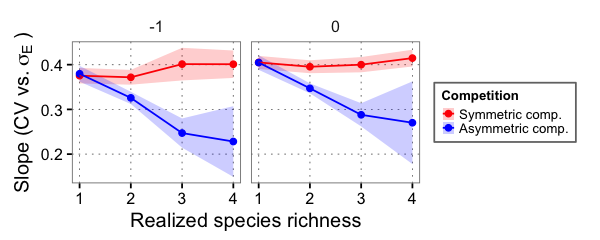
\includegraphics[width=5in]{./components/storage_effect_div+envar_varycomp_loglog_slopes.png}
  \caption{Slopes of linear fits for the relationship between log(\emph{CV}) and log($\sigma_E$) at different levels of realized species richness from storage effect simulations. The slopes come from linear models fit to log-transformed versions of Figure 3 in the main text. For these simulations, ``symmetric competion'' (\tikzcircle{1.5pt}) refers to similar live-to-dormant biomass allocation fractions ($\boldsymbol{\alpha} = [0.5, 0.495, 0.49, 0.485]$ for the four species), and ``asymmetric competition'' (\tikzcircle[fill=blue]{1.5pt}) refers to more dissimilar live-to-dormant biomass allocation fractions ($\boldsymbol{\alpha} = [0.5, 0.49, 0.48, 0.47]$ for the four species).}
\end{figure}

\newpage{}

\begin{figure}[!ht]
  \centering
      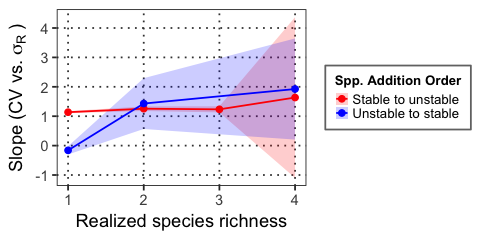
\includegraphics[width=5in]{./components/relative_nonlinearity_div+envar_loglog_slopes.png}
  \caption{Slopes of linear fits for the relationship between log(\emph{CV}) and log($\sigma_R$) at different levels of realized species richness from relative nonlinearity simulations. The slopes come from linear models fit to log-transformed versions of Figure 4 in the main text.}
\end{figure}

\hypertarget{refs}{}
\hypertarget{ref-Yuan2015}{}
Yuan, C. \& Chesson, P. (2015). The relative importance of relative
nonlinearity and the storage effect in the lottery model.
\emph{Theoretical Population Biology}, 105, 39--52.


\end{document}
